\begin{figure*}[tp]
  % from paper-rework/a1-layout-figure/ancilla-layouts-B.pdf, caption-layout-B.tex part 2 (restructure 2026-11-19)
  \centering
  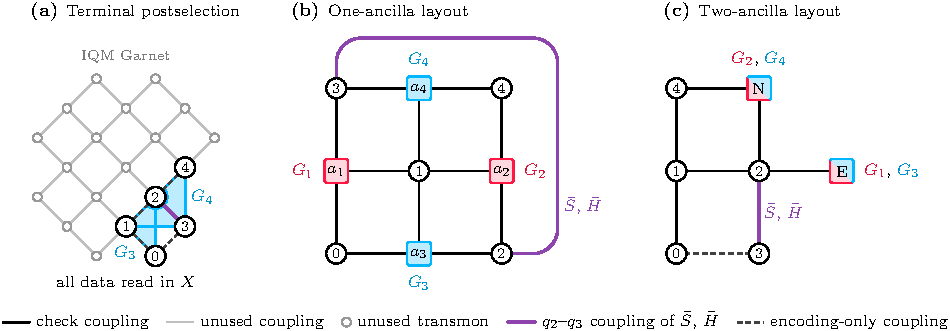
\includegraphics{figures/layouts-three.pdf}% drawn at final size
  \caption{Qutrits and couplings of the $[[5,1,2]]_3$ code in terminal postselection (a) and in the one-ancilla (b) and two-ancilla (c) layouts, with each coupling marked by its use in the stabilizer measurements, the logical gates or the encoding circuit. Circles with an index are data qutrits, small circles are unused transmons, and squares are ancillas. Red marks the $Z$-type stabilizers $G_1$, $G_2$ and blue the $X$-type $G_3$, $G_4$ (Eqs.~\eqref{eq:s1} and~\eqref{eq:s4}), and the label beside an ancilla names the stabilizers it measures in each check round. Dashed couplings are used only by the encoding circuit.
(a)~Terminal postselection on IQM's Garnet QPU, whose 20 transmons sit on a square lattice with 30 couplings between nearest neighbors~\cite{IQM240812433}. Drawn in the orientation of IQM's device map, with QB1 at the bottom, the transmons QB1, QB4, QB5, QB2 and QB6 hold $q_0, \dots, q_4$, respectively. The dashed couplings are the four that its encoding circuit uses (\autoref{fig:encoding_circuit}(a)). No ancillas are used, and the final $X$-basis readout of all data qutrits gives $G_3$ and $G_4$ (shaded; their blue outlines are not couplings, and that of $G_4$ bends around $q_2$).
(b)~One-ancilla layout on the conventional surface-code grid, with $q_1$ at the center. Ancilla $a_j$ neighbors the three data qutrits of $G_j$, and the two-qutrit gates of $\bar H$ and $\bar S$ (Eqs.~\eqref{eq:logical_H} and~\eqref{eq:logical_HS}) need a long-range coupling between $q_2$ and $q_3$. The encoding circuit of this layout (\autoref{fig:encoding_circuit}(b)) uses only check couplings, so this panel has no dashed coupling.
(c)~Two-ancilla layout: the ancillas N and E and eight couplings, all between nearest neighbors of a square lattice. N measures $G_2$ and then $G_4$, and E measures $G_1$ and then $G_3$, so each of their squares carries both colors. Neither ancilla is next to all three data qutrits of these stabilizers, so the extraction circuits (\autoref{fig:extraction_circuits}(e)--(h)) also apply SUM gates and their inverses between data qutrits, on $q_0$--$q_1$, $q_1$--$q_2$, $q_1$--$q_4$ and $q_2$--$q_3$, the coupling that also carries the two-qutrit gates of $\bar H$ and $\bar S$. The encoding circuit of this layout (\autoref{fig:encoding_circuit}(c)) uses the dashed coupling $q_0$--$q_3$ and three solid ones.}
  \label{fig:ancilla_layouts}
\end{figure*}
